\documentclass[../../main.tex]{subfiles}

\graphicspath{{../../image/}{../../figure/}}

\begin{document}

\section{深度学习的影响}\label{section:ch01-深度学习的影响}

机器学习是当今最重要、发展最快的技术领域之一。机器学习的应用遍及各个领域，基于数据学习的解决方案正逐步取代传统的手工设计算法。这不仅提升了现有技术的性能指标，更为一系列全新能力的开发打开了大门。而如果新算法仍需完全依赖人工设计，这些能力的实现将是无法想象的。

作为机器学习的一个分支，深度学习（Deep Learning, DL）已经成为一种异常强大且通用的数据学习框架。深度学习的理论基础是被称为神经网络（neural network）的计算模型，这些模型最初是受到人类大脑中学习和信息处理机制的启发而产生的。人工智能（Artificial Intelligence, AI）领域致力于在机器中重现人脑的强大能力，而今天“机器学习”和“人工智能”这两个术语常常被交替使用。当前使用的许多人工智能系统，实际上是机器学习的具体应用，旨在解决特定领域的问题。这些系统虽然非常有用，但与人类大脑的巨大能力相比仍有很大差距。人们引入了“通用人工智能”（Artificial General Intelligence, AGI）这一概念，来描述构建具有更高灵活性的智能系统的愿景。经过几十年的稳步发展，机器学习现在已进入快速发展阶段（参见\cref{chapter:ch12-Transformer与注意力机制}）。最近，一种称为大语言模型的庞大深度学习系统开始展现出卓越的能力，人们把这些能力视为通用人工智能的初步迹象（Bubeck et al., 2023）。

本节从4个不同领域的示例来讨论机器学习，以此说明这一技术应用的广泛性，同时引入一些相关的基本概念和术语。值得注意的是，这些示例以及很多其他示例都是使用深度学习这一基本框架的不同变体来解决的。这与传统方法形成了鲜明对比，在传统方法中，不同的应用需要采用各种迥异且高度专业的技术来处理。应当强调的是，我们选择的例子只代表了深度神经网络应用广度的一小部分，事实上，几乎所有需要计算的领域都正在或即将受益于深度学习的革命性影响。

\subsection{医疗诊断}\label{subsection:ch01-医疗诊断}

我们先来看看机器学习在皮肤癌诊断中的应用。黑色素瘤（melanoma）是最危险的一种皮肤癌，但如果发现得早，是可治愈的。\cref{figure:ch01-皮肤病变}展示了皮肤病变的示例图片，上面的一行图像是危险的恶性黑色素瘤，下面的一行图像是良性痣。显然，区分这两类图片具有极大的挑战性，几乎不可能通过人工编写出一个算法来实现对这些图像的准确分类。

这个问题已经通过深度学习得到成功解决（Esteva et al., 2017）。该解决方案是通过一组大型的病变图像集构建的，该图集称为训练集，其中每一幅图像都被标注为恶性或良性，标注的依据是对病变活检后得到的真实分类。训练集用来确定深度神经网络中约2500万个可调参数的取值。这个根据数据反馈的结果来设置参数值的过程称为学习或训练。训练的目标是使得训练好的神经网络根据新病变的图像就可以预测病变是良性还是恶性，而无须执行耗时的活检步骤。

\begin{definition}[训练集、权重与训练]\label{definition:ch01-训练集权重与训练}
设 $N\in\mathbb{N}$，$\mathcal{X}$ 为输入空间，$\mathcal{Y}$ 为目标空间，$\{(x_n,t_n)\}_{n=1}^{N}\in(\mathcal{X}\times\mathcal{Y})^{N}$ 为一组样本，其中 $x_n$ 为第 $n$ 个样本的输入，$t_n$ 为它对应的标注。若这组样本的每个输入 $x_n$ 都配有标注 $t_n$，则它称为\textbf{训练集}（training set），$x_n$ 称为输入变量，$t_n$ 称为目标变量或标签，$N$ 称为训练集的样本数。

设 $P\in\mathbb{N}$ 为参数个数，参数空间 $\mathcal{W}\subseteq\mathbb{R}^{P}$，模型由映射 $y(\cdot;\mathbf{w}):\mathcal{X}\to\mathcal{Y}$ 与参数 $\mathbf{w}\in\mathcal{W}$ 给出，则 $\mathbf{w}$ 称为该模型的\textbf{权重}（weight）。设 $\mathcal{A}:(\mathcal{X}\times\mathcal{Y})^{N}\to\mathcal{W}$ 为映射，若 $\mathbf{w}$ 按
\begin{align*}
  \mathbf{w}=\mathcal{A}\bigl((x_1,t_1),\dots,(x_N,t_N)\bigr)
\end{align*}
取值，则 $\mathcal{A}$ 称为\textbf{学习算法}（learning algorithm），按 $\mathcal{A}$ 由训练集确定 $\mathbf{w}$ 的过程称为\textbf{学习}（learning）或\textbf{训练}（training）。
\end{definition}

这是一个典型的监督学习问题的例子，因为在训练过程中，每个样本都标注了正确的类别标签。这同时也是一个分类问题的例子，因为每个输入经过处理后，都需要被分配到离散的类别集合中（本例中为“良性”或“恶性”）。如果输出包括一个或多个连续变量，则称为回归问题。在化工生产过程中，根据温度、压力和反应物浓度预测产量，就是回归问题的一个例子。

\begin{definition}[监督学习、分类与回归]\label{definition:ch01-监督学习分类与回归}
设 $N\in\mathbb{N}$，输入空间 $\mathcal{X}$，目标空间 $\mathcal{Y}$，训练集 $\{(x_n,t_n)\}_{n=1}^{N}\subseteq\mathcal{X}\times\mathcal{Y}$，参数空间 $\mathcal{W}\subseteq\mathbb{R}^{P}$（$P\in\mathbb{N}$），学习算法 $\mathcal{A}$ 按\cref{definition:ch01-训练集权重与训练}由训练集确定权重 $\mathbf{w}\in\mathcal{W}$。
\begin{enumerate}
  \item 若训练只使用样本对 $(x_n,t_n)$，且对每个 $n$ 目标值 $t_n$ 为已知，则相应的学习问题称为\textbf{监督学习}（supervised learning）；
  \item 在监督学习中，若目标空间 $\mathcal{Y}$ 为有限集，则称该问题为\textbf{分类}（classification）问题，$\mathcal{Y}$ 的每个元素称为一个\textbf{类别}（class）；
  \item 在监督学习中，若 $\mathcal{Y}\subseteq\mathbb{R}^{K}$（$K\in\mathbb{N}$，$K\geqslant1$）且目标值取连续值，则称该问题为\textbf{回归}（regression）问题，$K$ 称为输出的维数。
\end{enumerate}
\end{definition}

这个应用的一个有趣之处是，可用的带标注的训练图像数量相对较少，大约只有12.9万幅。因此，研究人员首先要在一个包含128万幅日常物体（如狗、建筑和蘑菇等）图像的大型数据集上对深度神经网络进行预训练，然后在皮肤病变图像数据集上对进行微调。这是迁移学习的一个例子，神经网络从日常物体的大规模数据集中学习自然图像的一般属性，随后专门针对皮肤病变分类问题进行优化。使用深度学习技术对皮肤病变图像进行分类的准确率已经超过专业皮肤科医生的水平（Brinker et al., 2019）。

\begin{definition}[预训练、微调与迁移学习]\label{definition:ch01-预训练微调与迁移学习}
设源任务 $\mathcal{T}_{\mathrm{s}}$ 的训练集为 $\mathcal{D}_{\mathrm{s}}\subseteq\mathcal{X}_{\mathrm{s}}\times\mathcal{Y}_{\mathrm{s}}$，目标任务 $\mathcal{T}_{\mathrm{t}}$ 的训练集为 $\mathcal{D}_{\mathrm{t}}\subseteq\mathcal{X}_{\mathrm{t}}\times\mathcal{Y}_{\mathrm{t}}$，两个任务的数据分布不必相同；参数空间 $\mathcal{W}\subseteq\mathbb{R}^{P}$（$P\in\mathbb{N}$），学习算法 $\mathcal{A}:\mathcal{P}(\mathcal{X}\times\mathcal{Y})\times\mathcal{W}\to\mathcal{W}$ 以数据集与初始权重为输入、以权重为输出，其中 $\mathcal{P}(\cdot)$ 表示幂集，$\mathbf{w}_{\mathrm{init}}\in\mathcal{W}$ 为初始权重。
\begin{enumerate}
  \item 若 $\mathbf{w}_{0}=\mathcal{A}(\mathcal{D}_{\mathrm{s}},\mathbf{w}_{\mathrm{init}})$，即权重由源任务数据确定，则这一阶段称为\textbf{预训练}（pre-training），$\mathcal{D}_{\mathrm{s}}$ 称为\textbf{源数据集}；
  \item 若以 $\mathbf{w}_{0}$ 为初值在目标任务数据上继续训练，即 $\mathbf{w}_{1}=\mathcal{A}(\mathcal{D}_{\mathrm{t}},\mathbf{w}_{0})$，则这一阶段称为\textbf{微调}（fine-tune）；
  \item 若目标任务上的最终权重 $\mathbf{w}_{1}$ 由 $(\mathcal{D}_{\mathrm{s}},\mathcal{D}_{\mathrm{t}})$ 经上述两阶段得到，则这一做法称为\textbf{迁移学习}（transfer learning）。
\end{enumerate}
\end{definition}

\begin{figure}[htbp]
  \centering
  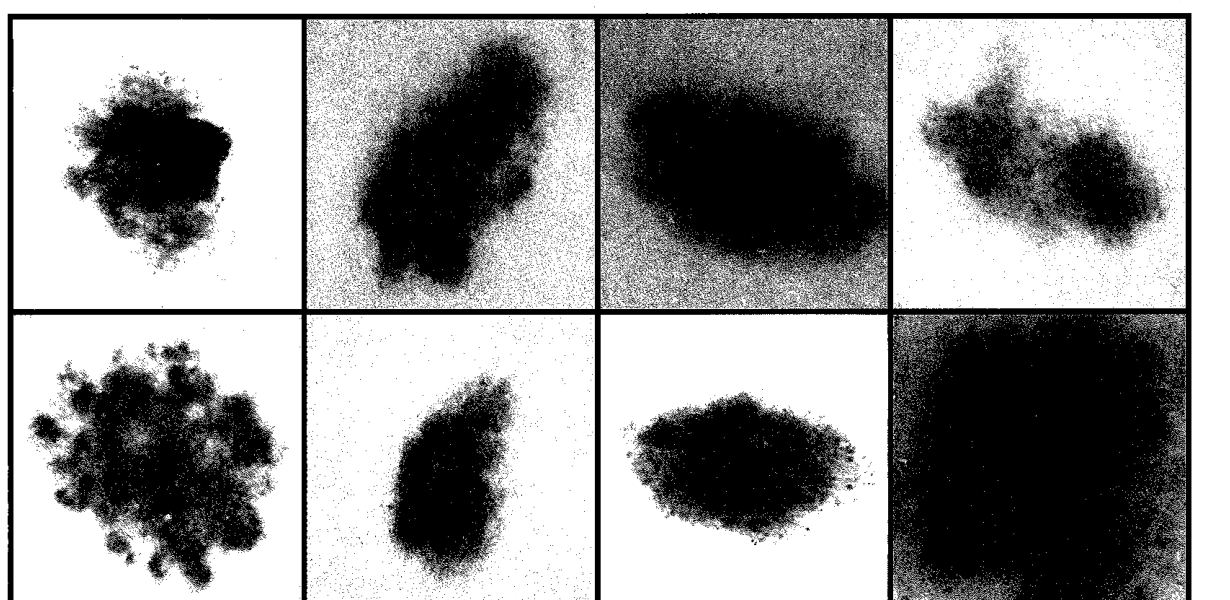
\includegraphics[width=0.85\textwidth]{ch01-fig1-1-skin-lesion.png}
  \caption{上面的一行图像是危险的恶性黑色素瘤，下面的一行图像是良性痣。未经专业训练的人很难区分这两类皮肤病变类型。}
  \label{figure:ch01-皮肤病变}
\end{figure}

% SUPPLEMENT: parent=definition:ch01-训练集权重与训练; kind=motivation; location=紧随其后的 remark
% SUPPLEMENT: parent=definition:ch01-监督学习分类与回归; kind=motivation; location=紧随其后的 remark
% SUPPLEMENT: parent=definition:ch01-预训练微调与迁移学习; kind=motivation; location=紧随其后的 remark
\begin{remark}
上面三个定义刻画了监督学习的三层结构：\cref{definition:ch01-训练集权重与训练}给出“数据与参数”，\cref{definition:ch01-监督学习分类与回归}按标签形态把任务分为分类与回归，\cref{definition:ch01-预训练微调与迁移学习}则说明了在标注数据稀缺时如何借助无关的大数据集。

“有标注”是监督学习的前提，它把“学习什么”变成了“拟合什么”：正因为每个 $x_n$ 都配有 $t_n$，训练才可以归结为让模型输出逼近已知目标值，才有了后文可以最小化的误差函数。分类与回归的区分不在于算法，而在于输出空间的形态——离散类别给出的是“判定”，连续变量给出的是“估计”，两者的损失函数与评价方式因此不同（详见\cref{chapter:ch05-分类}与\cref{chapter:ch04-回归}）。

迁移学习之所以成立，是因为自然图像的底层统计特性（边缘、纹理、颜色分布）在不同任务之间高度共享；预训练阶段学到的正是这些共性，微调阶段只需要调整与具体任务相关的部分。因此，微调的必要条件是两个任务的输入分布不能相差过远，否则预训练得到的 $\mathbf{w}_{0}$ 不再是良好的初值。
\end{remark}

\subsection{蛋白质结构预测}\label{subsection:ch01-蛋白质结构预测}

蛋白质常被称为生物体的基石。它们是由一个或多个氨基酸的长链组成的生物分子，蛋白质的特性则由22种不同类型的氨基酸序列所决定。当蛋白质在活细胞内合成后，就会折叠成复杂的三维结构，其行为和相互作用很大程度上取决于折叠的形态。

怎么根据氨基酸序列推导出蛋白质的三维结构呢？这是生物学界几十年来一直想攻克的基础性难题，但是进展甚微，直到深度学习技术带来了突破性进展。

蛋白质的三维结构可以通过X射线晶体学、低温电子显微镜或核磁共振光谱等实验技术进行测定。然而，这个过程通常非常耗时，而且对某些蛋白质来说，这种方法极具挑战性。例如，很难得到蛋白质的纯净样本，或者蛋白质的结构依赖于特定环境。相比之下，确定蛋白质的氨基酸序列的实验成本较低，产出较高。因此，如何直接从氨基酸序列预测蛋白质的三维结构引起广泛关注，这有助于更好地了解生物过程，以及用于新药研发等实际应用。我们可以以氨基酸序列为输入、以蛋白质的三维结构为输出来训练深度学习模型，其中的训练数据包含了已知的氨基酸序列和对应的蛋白质三维结构。因此，蛋白质结构预测也是监督学习的一个例子。经过训练的系统能够以新的氨基酸序列为输入，预测对应的蛋白质三维结构（Jumper et al., 2021）。\cref{figure:ch01-蛋白质结构}比较了一种蛋白质的预测三维结构和通过X射线晶体学获得的实际三维结构。

\begin{figure}[htbp]
  \centering
  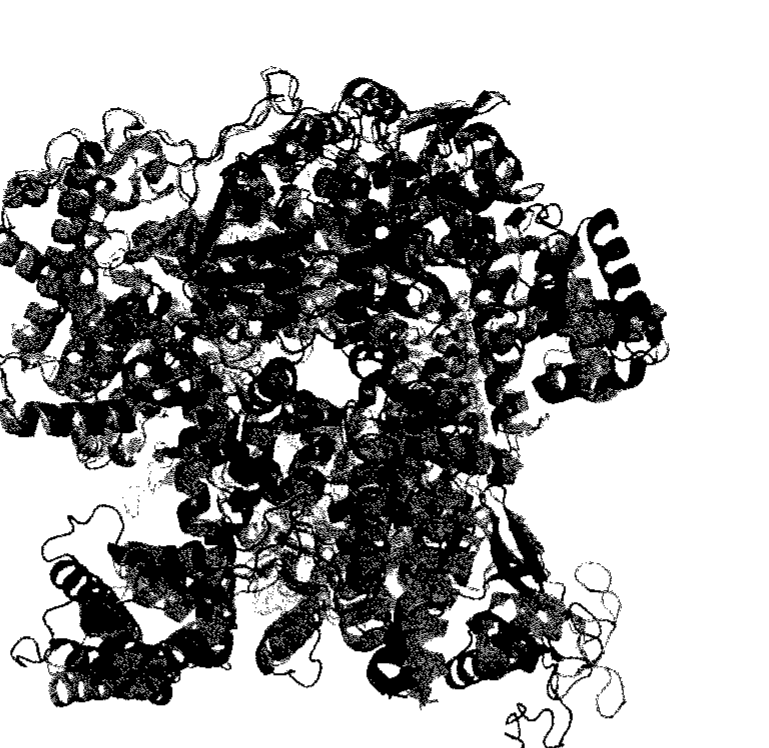
\includegraphics[width=0.5\textwidth]{ch01-fig1-2-protein-structure.png}
  \caption{一种名为T1044/6VR4的蛋白质的三维形状。绿色结构展示了通过X射线晶体学确定的真实三维结构，而叠加在上面的蓝色结构展示了深度学习模型AlphaFold预测的三维结构〔图片来源于Jumper et al. (2021)，经许可使用〕。}
  \label{figure:ch01-蛋白质结构}
\end{figure}

\begin{remark}本工程的全部插图都直接裁自原书扫描件，未重绘、未上色。该扫描件
是灰度图，原书的彩色插图在此以灰度深浅呈现；图题与正文中提到的颜色（红、绿、蓝、橙等）
沿用原书表述，请按原书的配色理解，而形状、线型、箭头与坐标标注仍然可辨。
\end{remark}

\subsection{图像合成}\label{subsection:ch01-图像合成}

在上面讨论的两个应用中，神经网络学会了将输入（皮肤图像或氨基酸序列）转换成输出（病变分类或蛋白质的三维结构）。现在我们来看一个不同的例子：训练数据是一组样本图像，训练后的神经网络能生成类似的新图像。与病变分类和蛋白质结构预测的例子不同，这些训练图像是没有标注的，这样的训练属于无监督学习。\cref{figure:ch01-生成人脸}展示了一些由深度神经网络生成的合成图像，该深度神经网络是在拍摄于摄影棚单色背景下的人脸图像集上进行训练的。这些合成图像质量极高，很难将它们和真人照片区分开来。

\begin{definition}[无监督学习]\label{definition:ch01-无监督学习}
设 $N\in\mathbb{N}$，输入空间 $\mathcal{X}$，参数空间 $\mathcal{W}\subseteq\mathbb{R}^{P}$（$P\in\mathbb{N}$），$x_1,\dots,x_N\in\mathcal{X}$ 为训练样本。若学习算法 $\mathcal{A}:\mathcal{X}^{N}\to\mathcal{W}$ 的输入只有 $x_1,\dots,x_N$，即训练不使用任何人工给出的目标值，则相应的学习问题称为\textbf{无监督学习}（unsupervised learning），$\mathcal{A}$ 称为无监督学习算法。
\end{definition}

这种模型可以生成与训练数据不同但又有类似统计特性的结果，所以被称为生成式模型。这种方法的一个变体能根据输入的文本字符串（称为提示词，prompt）生成反映文本语义的图像（参见\cref{chapter:ch10-卷积网络}）。我们用生成式AI（generative AI）这个术语来描述那些能生成图像、视频、音频、文本、候选药物分子或其他形态信息的深度学习模型。

\begin{definition}[生成式模型、提示词与生成式AI]\label{definition:ch01-生成式模型与提示词}
设样本空间 $\mathcal{X}\subseteq\mathbb{R}^{D}$（$D\in\mathbb{N}$），$(\Omega,\mathcal{F},\mathbb{P})$ 为概率空间，$X:\Omega\to\mathcal{X}$ 服从未知分布 $p_{\mathrm{data}}$，$x_1,\dots,x_N$ 为 $X$ 的 $N$ 个独立观测；设 $\{p_{\boldsymbol{\theta}}:\boldsymbol{\theta}\in\Theta\}$ 为一族 $\mathcal{X}$ 上的概率分布，其参数 $\boldsymbol{\theta}$ 由 $x_1,\dots,x_N$ 确定，$d$ 为 $\mathcal{X}$ 上概率分布之间的全变差距离。
\begin{enumerate}
  \item 给定容差 $\varepsilon\in(0,1)$。若 $d(p_{\boldsymbol{\theta}},p_{\mathrm{data}})\leqslant\varepsilon$ 且存在从 $p_{\boldsymbol{\theta}}$ 采样的算法，则 $\{p_{\boldsymbol{\theta}}\}$ 连同其采样过程称为\textbf{生成式模型}（generative model）；
  \item 设 $\Sigma$ 为有限字符集，$\Sigma^{*}$ 为 $\Sigma$ 上长度有限的字符串集合。若 $c\in\Sigma^{*}$ 作为条件输入模型，模型给出条件分布 $p_{\boldsymbol{\theta}}(\cdot\mid c)$ 并可由该分布采样，则 $c$ 称为\textbf{提示词}（prompt）；
  \item “生成式AI”是\textbf{非形式化术语}，其可操作版本为：设 $\mathcal{Z}$ 为某类内容的取值空间，若一个深度学习模型对每个 $c\in\Sigma^{*}$ 给出 $\mathcal{Z}$ 上的条件分布 $p_{\boldsymbol{\theta}}(\cdot\mid c)$ 并可由该分布采样，则它称为该内容空间上的\textbf{生成式模型}，这类模型的总称记为\textbf{生成式AI}（generative AI）。
\end{enumerate}
\end{definition}

\begin{figure}[htbp]
  \centering
  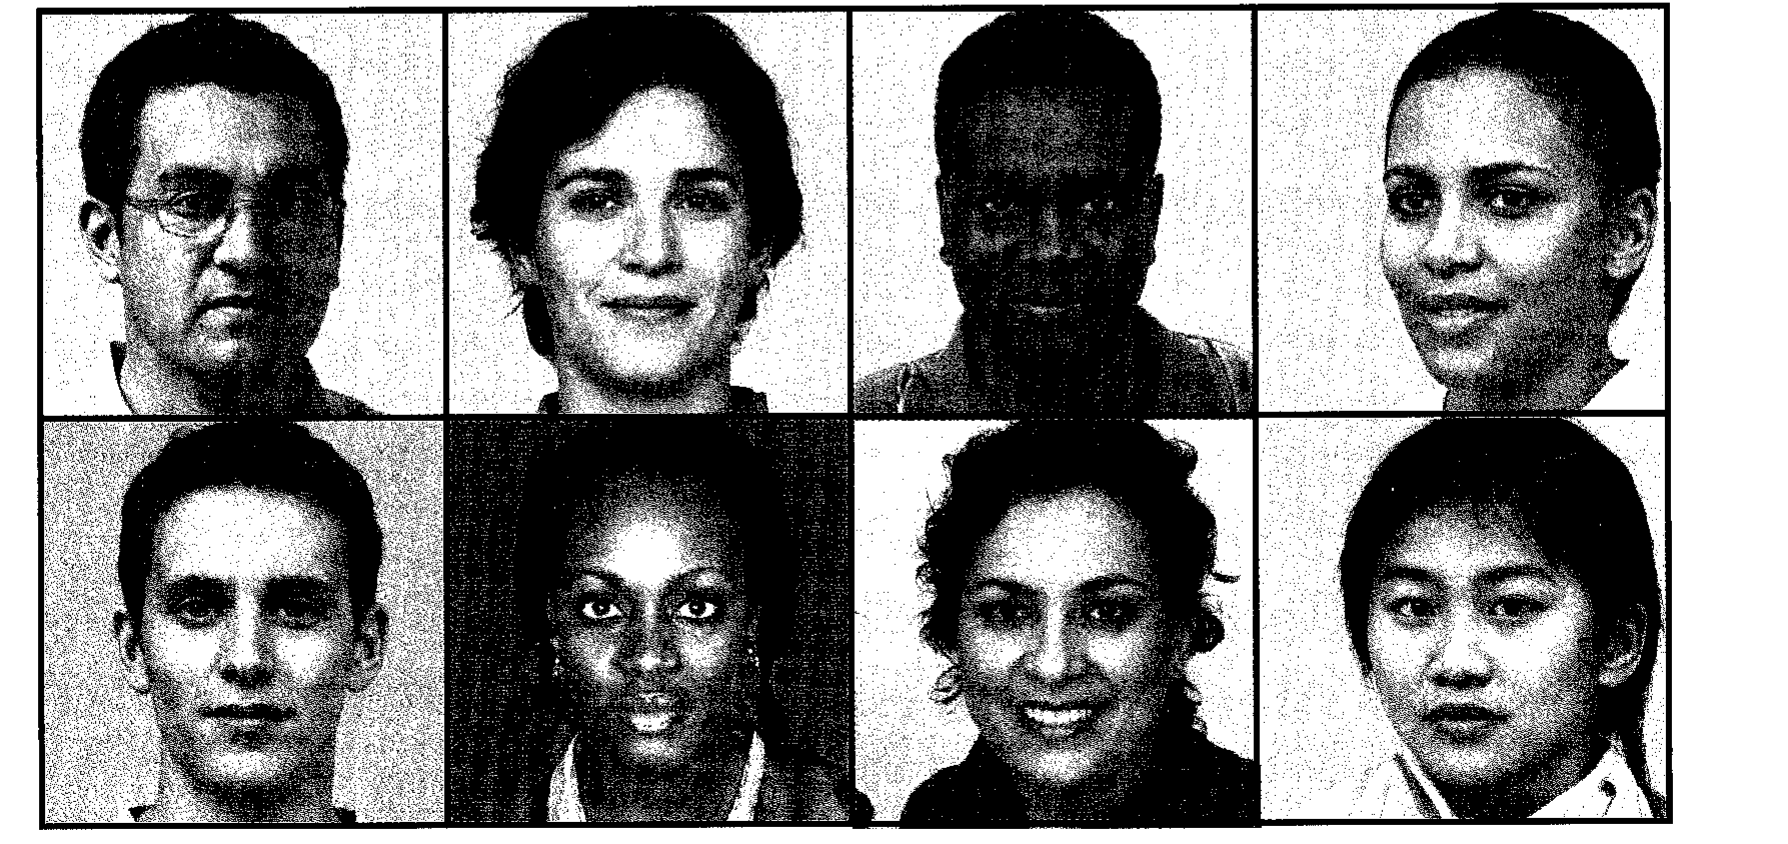
\includegraphics[width=0.85\textwidth]{ch01-fig1-3-generated-faces.png}
  \caption{由无监督学习方法训练得到的深度神经网络生成的人脸图像〔来自generated.photos网站〕。}
  \label{figure:ch01-生成人脸}
\end{figure}

% SUPPLEMENT: parent=definition:ch01-无监督学习; kind=motivation; location=紧随其后的 remark
% SUPPLEMENT: parent=definition:ch01-生成式模型与提示词; kind=motivation; location=紧随其后的 remark
\begin{remark}
\cref{definition:ch01-无监督学习}与\cref{definition:ch01-生成式模型与提示词}的差别，正是“判别”与“生成”的差别：前者只要求模型从数据中提取结构，后者要求模型能够从结构中重新采出样本。由于没有标签可以把“错”定义成“与 $t_n$ 不一致”，无监督学习必须以数据分布本身为学习目标，这既是它的困难所在，也是它能够被用于生成的原因。

定义中的“新样本”指从 $p_{\boldsymbol{\theta}}$ 独立抽取的样本，并不要求它与训练集逐点不同：在连续分布下，新样本与任一训练样本重合的概率为零；在离散分布下则允许以正概率重复训练样本，这正是语言模型可以逐字复现训练文本的原因。容差 $\varepsilon$ 是模型选择时给定的精度指标，不是“存在某个 $\varepsilon$”的存在性断言。

对生成式模型而言，“与训练数据不同但统计特性相似”这一条不能弱化为“与训练数据相同”：若模型只会复制训练样本，它就退化为查表，失去了泛化到新样本的能力；也不能强化为“必须复现 $p_{\mathrm{data}}$ 的每一个细节”，因为在有限样本下真实分布本身无法被精确恢复。提示词的存在说明条件生成是一般情形——模型学到的实际上是条件分布 $p(\text{图像}\mid\text{提示词})$，无条件生成只是提示词为空的特例。
\end{remark}

\subsection{大语言模型}\label{subsection:ch01-大语言模型}

近年来，机器学习领域最重要的进展之一，是研发人员开发出了强大的模型来处理自然语言和类似程序代码这样的序列数据。大语言模型利用深度学习技术构建丰富的内部表征，捕捉语言的语义属性。

\begin{definition}[大语言模型]\label{definition:ch01-大语言模型}
设 $\mathcal{V}$ 为有限词表，$\mathcal{V}^{*}=\bigcup_{T\geqslant1}\mathcal{V}^{T}$ 为 $\mathcal{V}$ 上长度有限的词序列集合，$\Delta(\mathcal{V})$ 为 $\mathcal{V}$ 上的概率单纯形，$L\in\mathbb{N}$ 为参数个数，$\boldsymbol{\theta}\in\mathbb{R}^{L}$ 为参数，$p_{\boldsymbol{\theta}}:\mathcal{V}^{*}\to\Delta(\mathcal{V})$ 为把词序列映为下一个词的概率分布的映射。
“大语言模型”是\textbf{非形式化术语}，其可操作版本为：若
\begin{enumerate}
  \item $p_{\boldsymbol{\theta}}$ 由有限个可微层复合而成；
  \item 参数个数 $L$ 与预训练语料规模均大于预先给定的阈值；
  \item 对每个 $T\geqslant1$ 与每个 $w_{1:T}=(w_{1},\dots,w_{T})\in\mathcal{V}^{T}$，模型给出条件分布 $p_{\boldsymbol{\theta}}(\cdot\mid w_{1:T})\in\Delta(\mathcal{V})$ 并可由该分布采样，
\end{enumerate}
则该模型称为\textbf{大语言模型}（Large Language Model, LLM）。其中“丰富的内部表征”“语义属性”属于非形式化描述，本定义不赋予其独立含义。
\end{definition}

有一类重要的大语言模型称为自回归（autoregressive）语言模型，它们能够输出语言，因此属于生成式AI的一种。这类模型以一个词序列作为输入，生成这个词序列最可能的下一个词，我们可以把末尾添加了新词的扩展序列再输入到模型中，让它生成后续的词，重复这个过程，就会得到越来越长的词序列。这样的模型还可以输出一个特殊的“停止”词，来表示文本生成的结束，这样就使得模型在输出一定长度的文本后停止。此时，用户可以在词序列的末尾添加自定义的词序列，然后将完整的词序列重新输入模型以触发生成后续的词。通过这种方式，人们就可以和神经网络对话了。

\begin{definition}[自回归语言模型]\label{definition:ch01-自回归语言模型}
设 $\mathcal{V}$ 为有限词表，$\mathcal{V}^{*}=\bigcup_{T\geqslant1}\mathcal{V}^{T}$，$p_{\boldsymbol{\theta}}:\mathcal{V}^{*}\to\Delta(\mathcal{V})$ 为参数 $\boldsymbol{\theta}\in\mathbb{R}^{L}$ 给出的条件分布，其中 $p_{\boldsymbol{\theta}}(w\mid w_{1:t})$ 表示前缀为 $w_{1:t}=(w_{1},\dots,w_{t})$ 时下一个词为 $w$ 的概率，$w_{1:0}$ 表示空序列。若对每个 $T\geqslant1$ 与每个 $w_{1:T}\in\mathcal{V}^{T}$ 有
\begin{align*}
  p_{\boldsymbol{\theta}}(w_{1:T})=\prod_{t=1}^{T}p_{\boldsymbol{\theta}}(w_{t}\mid w_{1:t-1}),
\end{align*}
则相应的模型称为\textbf{自回归语言模型}（autoregressive language model）。给定前缀 $w_{1:t}$ 后，模型输出 $\hat{w}_{t+1}=\arg\max_{w\in\mathcal{V}}p_{\boldsymbol{\theta}}(w\mid w_{1:t})$；把 $\hat{w}_{t+1}$ 接到序列末尾得到 $w_{1:t+1}$ 并重复该步骤，所得序列的长度随步数严格增加。若 $\mathcal{V}$ 含特殊词 $\langle\mathrm{stop}\rangle$ 且 $\hat{w}_{t+1}=\langle\mathrm{stop}\rangle$，则称生成为\textbf{终止}。
\end{definition}

这类模型可以在大型文本数据集上通过提取训练对（training pair）进行训练。训练对的输入是随机选定的词序列，输出是已知的下一个词。这是自监督学习的一个例子，在自监督学习中，模型学习从输入到输出映射函数，有标注的输出是从输入训练数据中自动获取的，无须进行另外的人工标注。这种方法能把多种来源的大量文本作为大型训练集，从而训练出超大规模神经网络。

\begin{definition}[训练对与自监督学习]\label{definition:ch01-自监督学习}
设 $N\in\mathbb{N}$，输入空间 $\mathcal{X}$，目标空间 $\mathcal{Y}$，$g:\mathcal{X}\to\mathcal{Y}$ 为固定的、由数据生成方式确定的映射，$x_1,\dots,x_N\in\mathcal{X}$。若第 $n$ 个训练样本为 $(x_n,t_n)$ 且 $t_n=g(x_n)$ 由 $x_n$ 经 $g$ 自动得到、无须人工标注，则这样的样本对称为\textbf{训练对}（training pair），$g$ 称为\textbf{自监督目标}。若学习算法 $\mathcal{A}:(\mathcal{X}\times\mathcal{Y})^{N}\to\mathcal{W}$ 只以 $\{(x_n,g(x_n))\}_{n=1}^{N}$ 为输入来确定权重 $\mathbf{w}\in\mathcal{W}\subseteq\mathbb{R}^{P}$（$P\in\mathbb{N}$），则这一学习方式称为\textbf{自监督学习}（self-supervised learning）。
\end{definition}

一些专家认为，展现出非凡能力的大语言模型是通用人工智能的雏形（Bubeck et al., 2023），本书后面将详细讨论这类模型（参见\cref{chapter:ch12-Transformer与注意力机制}）。接下来，我们给出一个基于GPT-4（OpenAI, 2023）的语言生成示例。GPT-4能够针对如下提示做出响应：“请以莎士比亚戏剧风格，通过两个角色对话展开争论的方式证明素数有无穷多个”，其输出的译文见本页脚注。\footnote{译者用大模型翻译的原文图1.4（原书此处为截图）：\\
\textbf{甲}：汝未悟友啊，真理难准，素数无尽，犹如天辰。数不可分，纯而且简，虽觉奇迹，实则无边。\\
\textbf{乙}：可汝何以断定此论？何证可显，真理之根？\\
\textbf{甲}：听我言，疑心伴侣，一证妙绝，将疑云除。设若终极素数存在，为我们所见最大数领。名之“P”字，记于案头，构思新数“Q”，令人惊叹。它将超越“P”，成为素环。\\
\textbf{乙}：此证何从？友啊说明，胜利之杯，尚未高举。\\
\textbf{甲}：如斯简单，静待佳音，乘素数列，答案必寻。自二至“P”，逐一相连，得“Q”新数，正解现身。加一以固，使证更真，举证眼前，不再沉吟。\\
\textbf{乙}：现明白矣，如光闪莹，“Q”当素数，结论清晰。它不被小素整除有据，时序内自身是最大。既然选“P”作为终章，预设破碎，成为往昔。无终素数，真理已昭，数字无穷，如星海常在。}

% SUPPLEMENT: parent=definition:ch01-大语言模型; kind=motivation; location=紧随其后的 remark
% SUPPLEMENT: parent=definition:ch01-自回归语言模型; kind=motivation; location=紧随其后的 remark
% SUPPLEMENT: parent=definition:ch01-自监督学习; kind=motivation; location=紧随其后的 remark
\begin{remark}
\cref{definition:ch01-大语言模型}、\cref{definition:ch01-自回归语言模型}与\cref{definition:ch01-自监督学习}共同说明了为什么语言建模可以“无标签”地完成：自回归模型把第 $t+1$ 个词当作前 $t$ 个词的标签，于是任何一个文本语料都自动变成了训练集。条件“输入是随机选定的词序列”保证了模型见到的是文本的多种上下文，而不是固定的前缀；“输出是已知的下一个词”则保证了每一步都有确定的目标，这正是自监督学习的定义所指。

“自回归”中的“自”强调预测依赖于模型自己此前生成的输出：推理时序列越接越长，模型每一步的条件都在变化，因此误差会逐步累积——这是后文讨论采样策略与大模型生成质量时必须回到的事实。
\end{remark}

\end{document}
